\section{Creazione dello smart contract}\label{creazionesmartcontract}
Prima di poter creare lo smart contract è necessario generare l'account Algorand Intecs SpA con il quale, potremo creare lo smart contract e richiamare i metodi di quest'ultimo. Per la creazione di un account è sufficiente avviare il programma intecs.py presente nella cartella \textit{intecs}. Al primo avvio, digitiamo NO in quanto bisogna prima creare gli account Algorand che ci serviranno. Verrà quindi mostrata la schermata in figura \ref{fig: intecs_primoavvio }.
\begin{figure}[!h]
\flushleft
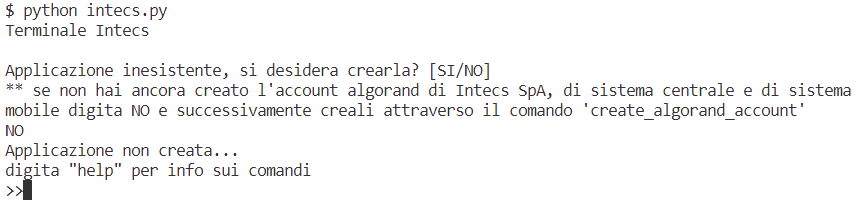
\includegraphics[scale=0.8]{images/Intecs/primo_avvio.png}
\caption{Primo avvio dell'interfaccia a linea di comando Intecs}
\label{fig: intecs_primoavvio }
\end{figure}\\
Attraverso il comando \textit{create\_algorand\_account} possiamo creare gli account Algorand.
\begin{figure}[!h]
\centering
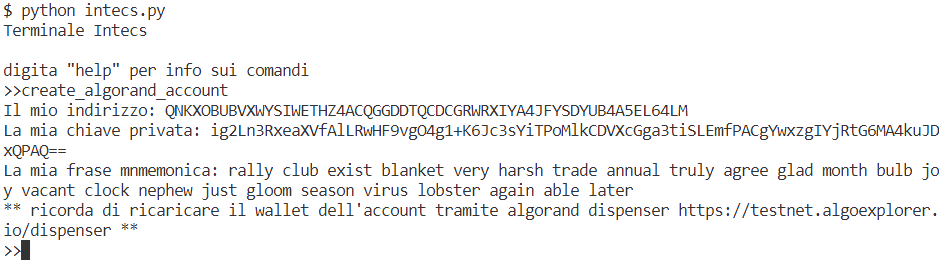
\includegraphics[scale=0.8]{images/Intecs/create_algorand_account_2.png}
\caption{Creazione degli account Algorand}
\label{fig: cli_creazioneaccount2 }
\end{figure}\\
Notiamo immediatamente dalla figura \ref{fig: cli_creazioneaccount2 } che la creazione di un account Algorand genera tre campi: l'indirizzo pubblico, la chiave privata e la mnemonica. E' necessario memorizzare manualmente questi dati visto che serviranno nelle fasi successive. Ricordiamo anche, che dopo la creazione di un account Algorand, il Wallet dovrà essere caricato con Algos (la moneta della TestNet) sfruttando l'Algorand Dispenser. Il comando \textit{create\_algorand\_account} va richiamato per creare l'account Intecs SpA, del sistema centrale e per ogni sistema mobile esistente. Nel nostro esempio consideriamo un solo sistema mobile. Una volta creato anche l'account di Intecs SpA chiudiamo il programma sfruttando il comando \textit{exit} per avere modo di modificare i valori delle variabili globali dell'account Algorand di Intecs (intecs\_address, intecs\_privatekey e intecs\_passphrase) che si trovano nelle prime righe del codice del programma subito dopo le librerie. Riavviamo nuovamente l'interfaccia a linea di comando intecs.py per effettuare finalmente l'operazione di creazione dello smart contract come nell'immagine \ref{fig: intecs_create_smart_contract}. 
\begin{figure}[!h]
\centering
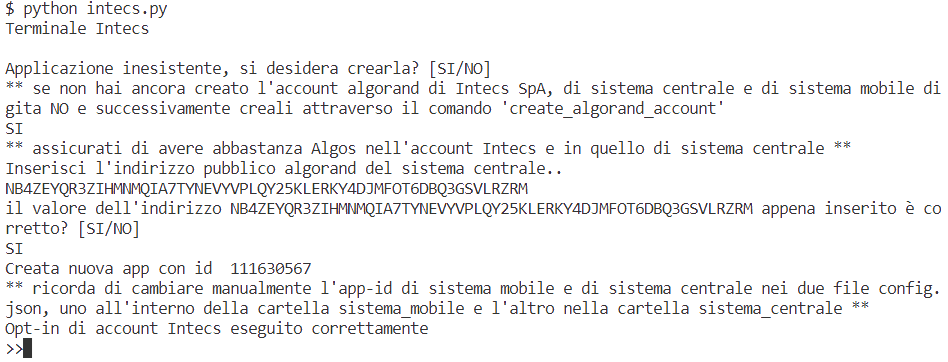
\includegraphics[scale=0.8]{images/Intecs/creazione_smartcontract.png}
\caption{Creazione dello smart contract}
\label{fig: intecs_create_smart_contract}
\end{figure}\\
L'operazione ha generato uno smart contract con il seguente ID: 111630567. Collegandosi al portale AlgoExplorer \cite{algoexplorer_testnet} e inserendo l'identificatore (ID) dello smart contract, possiamo verificare la corretta creazione di quest'ultimo.

\section{Setting dei file JSON}
Dopo la creazione dello smart contract è necessario andare a settare i valori degli account Algorand nel codice del programma di sistema centrale, di sistema mobile e di Cli v2. Più nel dettaglio:
\begin{itemize}
    \item apriamo il file info\_algorand.json presente nella cartella \textit{sistema\_centrale} per settare i tre parametri dell'indirizzo Algorand di sistema centrale (sistema\_centrale\_address, sistema\_centrale\_privatekey e sistema\_centrale\_passphrase) e il valore di app\_id, che sono stati generati nella sezione \ref{creazionesmartcontract}. Se non ricordiamo l'app-id associato allo smart contract creato, possiamo recuperarlo con il programma intecs.py richiamando il comando \textit{app-id}.
    \item apriamo il file info\_algorand.json presente nella cartella \textit{sistema\_mobile} per settare i tre parametri dell'indirizzo Algorand di sistema mobile (sistema\_mobile\_address, sistema\_mobile\_privatekey e sistema\_mobile\_passphrase) e il valore di app\_id  generati nella sezione \ref{creazionesmartcontract}. Nel caso in cui non ci si ricordi l'identificatore (id) associato allo smart contract creato, possiamo avviare il programma intecs.py e richiamare il comando \textit{app-id}, il quale restituirà il valore associato all'applicazione (smart contract).
    \item nella cartella \textit{cli v2} apriamo il file config.json e settiamo il valore della chiave sistema\_centrale\_address con l'indirizzo Algorand pubblico generato nella sezione \ref{creazionesmartcontract}.
\end{itemize}
Tutti i settaggi sono stati ora impostati correttamente.

\section{Avvio del programma}
L'avvio del programma è un'operazione che può essere istanziata automaticamente attraverso il docker-compose.yml con il comando \textit{docker-compose up --build}. Per sfruttare questa opzione è necessario aver installato sia Docker che Docker Compose. Nel qual caso si vogliano avviare manualmente le singole componenti senza far uso di Docker, è necessario prima di tutto modificare il campo \textit{host} delle configurazioni TCP, inserendo indirizzi IP validi al posto dei nomi di dominio impostati. Spieghiamo meglio questo concetto prendendo come esempio la configurazione utilizzata per la comunicazione TCP con il sistema mobile, ci riferiamo cioè al programma sistemacentrale.py, che gestisce la ricezione dei file zip e JSON. Notiamo che l'host, non è stato dichiarato sfruttando un indirizzo IP ma direttamente con il nome del servizio "sistemacentrale" dichiarato nel file docker-compose.yml il quale si riferisce al programma sistemacentrale.py e cioè al container del sistema centrale. Quest'operazione è consentita grazie a Docker Compose. Infatti quando nel docker-compose.yml aggiungiamo un servizio, non facciamo altro che definire un nuovo container e il nome stesso del container rappresenterà il suo nome di dominio.
\begin{pythoncode}
#configurazione Server TCP con Sistema Mobile (ricezione zip e json)
host_sm = "sistemacentrale"
port_sm = 12370
\end{pythoncode}
Questa proprietà vale però solo all'interno della rete Docker avviando il programma con docker-compose.yml. Nel qual caso si vogliano avviare le singole componenti manualmente (senza usare Docker) dobbiamo modificare tutte le varie configurazioni ed utilizzare indirizzi IP al posto dei nomi dei container per il campo \textit{host}. Le componenti poi dovranno essere avviate nel seguente ordine: sistemacentrale.py, sistemamobile.py e stazioneriferimento.py. In figura \ref{fig: sistemacentraleoutput } mostriamo l'output del sistema centrale subito dopo il suo avvio.
\begin{figure}[!h]
\flushleft
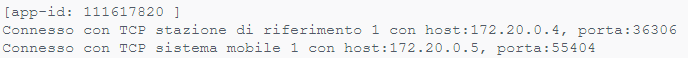
\includegraphics[scale=1.1]{images/simulazione/outputsistemacentrale.png}
\caption{Output dopo l'avvio del sistema centrale}
\label{fig: sistemacentraleoutput }
\end{figure}\\
Dopo aver avviato le tre componenti appena citate deve essere avviato il programma antenna che genererà il timestamp e lo invierà al sistema mobile e alla stazione di riferimento [vedi figura \ref{fig: antennaoutput }].
\begin{figure}[!h]
\flushleft
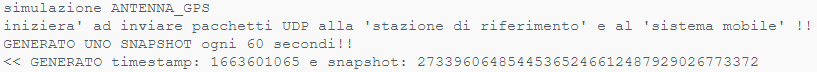
\includegraphics[scale=1.0]{images/simulazione/antennaoutput}
\caption{Output di antenna dopo l'invio di uno snapshot}
\label{fig: antennaoutput }
\end{figure}\\
L'output del terminale del sistema mobile conterrà la notifica di ricezione dello snapshot e del timestamp e mostrerà lo snapshot e i dati di posizioni appena generati [vedi figura \ref{fig: sistemamobile }].
\begin{figure}[!h]
\flushleft
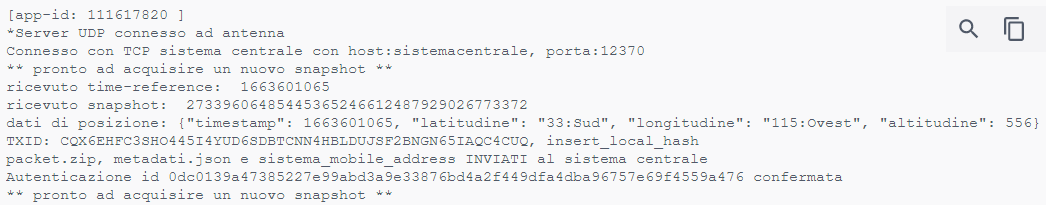
\includegraphics[scale=0.8]{images/simulazione/outputsistemamobile.png}
\caption{Schermata del sistema mobile}
\label{fig: sistemamobile }
\end{figure}\\
Anche il terminale della stazione di riferimento, avrà un output molto simile a quello del sistema mobile, conterrà infatti la notifica di ricezione del timestamp e dello snapshot e mostrerà lo snapshot e i dati di posizione appena generati [vedi figura \ref{fig: sistema_centrale6 }].\\
\begin{figure}[!h]
\flushleft
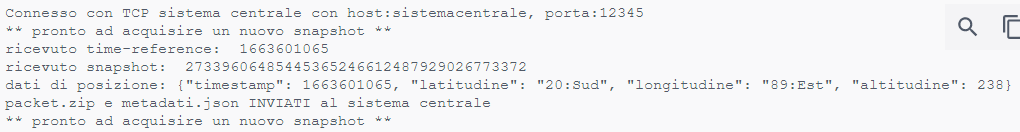
\includegraphics[scale=0.8]{images/simulazione/outputstazioneriferimento.png}
\caption{Schermata della stazione di riferimento}
\label{fig: sistema_centrale6 }
\end{figure}\\
Come ultima operazione, il sistema mobile e la stazione di riferimento inviano entrambi il file zip e il file JSON al sistema centrale sfruttando la comunicazione TCP. Dopo la ricezione di questi documenti, il sistema mobile invia anche il proprio indirizzo pubblico Algorand [vedi figura \ref{fig: sistema_centrale7 }]. 
\begin{figure}[!h]
\flushleft
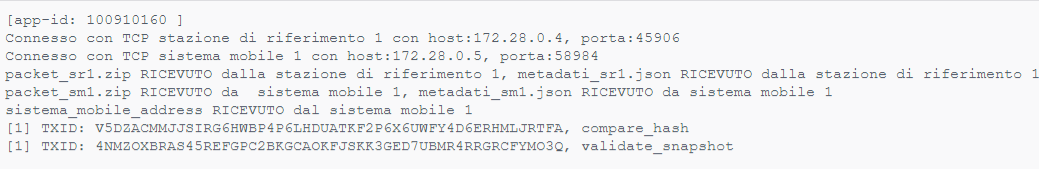
\includegraphics[scale=0.8]{images/simulazione/sistema_centrale.png}
\caption{Schermata del sistema centrale}
\label{fig: sistema_centrale7 }
\end{figure}
A questo punto, apriamo il programma Cli e sfruttiamo il comando \textit{stampa\_lista\_id} per vedere che l'id associato allo snapshot ricevuto poco fa dal sistema mobile ed inviato al sistema centrale è disponibile alla visualizzazione. Possiamo anche visualizzare alcune informazioni utili come la data e l'ora di ricezione dello snapshot da parte del sistema mobile e se lo snapshot è stato certificato correttamente. Quest'ultimo campo è rappresentato con un valore booleano True/False, ricordando che il valore booleano della validazione è settato a False se lo snapshot catturato dal sistema mobile e dalla stazione di riferimento non risultano equivalenti [vedi figura \ref{fig: sistema_centrale8 }].
\begin{figure}[!h]
\flushleft
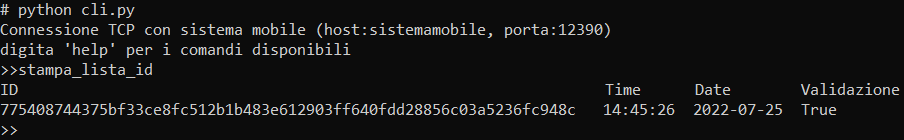
\includegraphics[scale=0.8]{images/simulazione/cli1.png}
\caption{Un primo esempio dell'interfaccia a linea di comando Cli}
\label{fig: sistema_centrale8 }
\end{figure}\\
Sfruttando il comando \textit{info\_id} e utilizzando come parametro l'id restituito da \textit{stampa\_lista\_id} possiamo avere accesso a tutte le informazioni associate allo snapshot corrispondente all'id passato. Diventa utile per ricercare un particolare snapshot catturato dal sistema mobile e controllare dove si trovava il sistema mobile ad una certa ora di un dato giorno [vedi figura \ref{fig: sistema_centrale9 }].
\begin{figure}[!h]
\flushleft
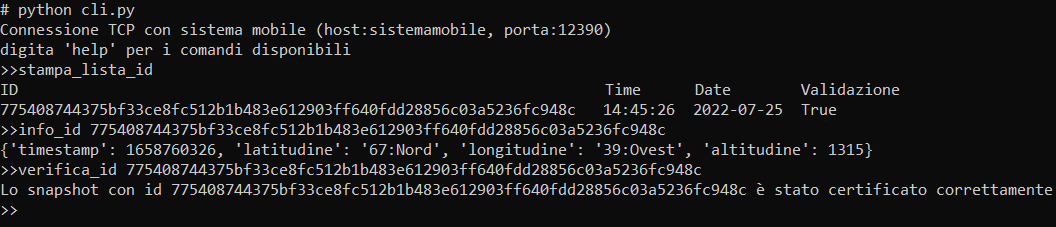
\includegraphics[scale=0.7]{images/simulazione/cli2.png}
\caption{Un secondo esempio dell'interfaccia a linea di comando Cli}
\label{fig: sistema_centrale9 }
\end{figure}